\documentclass[a4paper,twoside]{article}
\usepackage[T1]{fontenc}
\usepackage[bahasa]{babel}
\usepackage{graphicx}
\usepackage{graphics}
\usepackage{float}
\usepackage[cm]{fullpage}
\pagestyle{myheadings}
\usepackage{etoolbox}
\usepackage{setspace} 
\usepackage{lipsum} 
\setlength{\headsep}{30pt}
\usepackage[inner=2cm,outer=2.5cm,top=2.5cm,bottom=2cm]{geometry} %margin
% \pagestyle{empty}

\makeatletter
\renewcommand{\@maketitle} {\begin{center} {\LARGE \textbf{ \textsc{\@title}} \par} \bigskip {\large \textbf{\textsc{\@author}} }\end{center} }
\renewcommand{\thispagestyle}[1]{}
\markright{\textbf{\textsc{Laporan Perkembangan Pengerjaan Skripsi\textemdash Sem. Ganjil 2019/2020}}}

\onehalfspacing
 
\begin{document}

\title{\@judultopik}
\author{\nama \textendash \@npm} 

%ISILAH DATA BERIKUT INI:
\newcommand{\nama}{Chris Eldon}
\newcommand{\@npm}{2016730073}
\newcommand{\tanggal}{19/11/2019} %Tanggal pembuatan dokumen
\newcommand{\@judultopik}{Privacy Preserving Data Mining dengan Metode Randomization} % Judul/topik anda
\newcommand{\kodetopik}{MTA4703}
\newcommand{\jumpemb}{1} % Jumlah pembimbing, 1 atau 2
\newcommand{\pembA}{Mariskha Tri Adithia, P.D.Eng}
\newcommand{\pembB}{-}
\newcommand{\semesterPertama}{47 - Ganjil 19/20} % semester pertama kali topik diambil, angka 1 dimulai dari sem Ganjil 96/97
\newcommand{\lamaSkripsi}{1} % Jumlah semester untuk mengerjakan skripsi s.d. dokumen ini dibuat
\newcommand{\kulPertama}{Skripsi 1} % Kuliah dimana topik ini diambil pertama kali
\newcommand{\tipePR}{B} % tipe progress report :
% A : dokumen pendukung untuk pengambilan ke-2 di Skripsi 1
% B : dokumen untuk reviewer pada presentasi dan review Skripsi 1
% C : dokumen pendukung untuk pengambilan ke-2 di Skripsi 2

% Dokumen hasil template ini harus dicetak bolak-balik !!!!

\maketitle

\pagenumbering{arabic}

\section{Data Skripsi} %TIDAK PERLU MENGUBAH BAGIAN INI !!!
Pembimbing utama/tunggal: {\bf \pembA}\\
Pembimbing pendamping: {\bf \pembB}\\
Kode Topik : {\bf \kodetopik}\\
Topik ini sudah dikerjakan selama : {\bf \lamaSkripsi} semester\\
Pengambilan pertama kali topik ini pada : Semester {\bf \semesterPertama} \\
Pengambilan pertama kali topik ini di kuliah : {\bf \kulPertama} \\
Tipe Laporan : {\bf \tipePR} -
\ifdefstring{\tipePR}{A}{
			Dokumen pendukung untuk {\BF pengambilan ke-2 di Skripsi 1} }
		{
		\ifdefstring{\tipePR}{B} {
				Dokumen untuk reviewer pada presentasi dan {\bf review Skripsi 1}}
			{	Dokumen pendukung untuk {\bf pengambilan ke-2 di Skripsi 2}}
		}
		
\section{Latar Belakang}
Dengan semakin banyaknya penambangan data yang dilakukan dan data yang digunakan juga semakin banyak, semakin banyak juga privasi di dalam data tersebut yang tersebar kepada pihak yang melakukan penambangan data. Data privasi tersebut dapat tersebar kepada pihak yang tidak bertanggung jawab dan disalahgunakan. Oleh karena itu perlu adanya suatu cara untuk mencegah privasi tersebar pada proses penambangan data, menjaga privasi pada data tersebut. Istilah untuk hal tersebut adalah \textit{privacy preserving data mining}.

Salah satu cara untuk melakukan \textit{privacy preserving data mining} adalah dengan melakukan modifikasi data yang ada sebelum diberikan kepada pihak lain. Ada macam-macam teknik dan algoritma yang bertujuan modifikasi data untuk \textit{privacy preserving data mining} yang bisa dibagi menjadi dua jenis yaitu \textit{Perturbation Approach} dan \textit{Anonymization Approach}. \textit{Perturbation Approach} adalah pendekatan untuk \textit{privacy preserving data mining} dengan cara mengacaukan data yang ada, tetapi hasil data yang dikacaukan masih tetap bisa ditambang. \textit{Perturbation Approach} bisa dibagi menjadi dua jenis yaitu \textit{Value-based Perturbation Techniques} dan \textit{Multi-Dimensional Perturbation}.

\textit{Value-based Perturbation Techniques} adalah teknik yang bekerja dengan cara menyisipkan \textit{random noise} pada data. Sedangkan terdapat dua jenis teknik \textit{Multi-Dimensional Perturbation} yaitu \textit{Data mining Task-based Perturbation} dan \textit{Dimension Reduction-based Perturbation}. \textit{Data mining Task-based Perturbation} adalah teknik yang bekerja dengan cara modifikasi data sehingga properti yang bertahan pada data yang telah dimodifikasi spesifik hanya properti yang digunakan oleh suatu teknik penambangan data tertentu. Sedangkan \textit{Dimension Reduction-based Perturbation} adalah teknik yang bekerja dengan cara modifikasi data sekaligus mengurangi dimensi dari data asli.

\begin{figure}
	\centering
	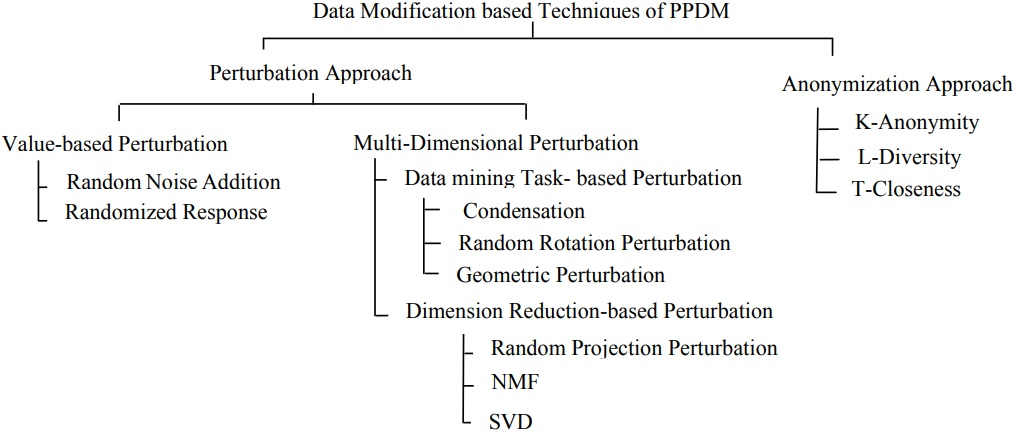
\includegraphics[scale=0.56]{ppdm}
	\caption{Berbagai macam teknik modifikasi data untuk \textit{privacy preserving data mining}}
	\label{fig:ppdm}
\end{figure}

Dari berbagai macam teknik modifikasi data untuk \textit{privacy preserving data mining} yang dapat dilihat pada Gambar \ref{fig:ppdm}, terdapat empat teknik yang menggunakan metode \textit{Randomization} yaitu \textit{Random Noise Addition}, \textit{Randomized Response}, \textit{Random Rotation Perturbation}, dan \textit{Random Projection Perturbation}.

Pada penelitian ini, akan dibuat sebuah perangkat lunak yang dapat memproses data yang akan ditambang menjadi data yang telah dimodifikasi dengan metode \textit{Randomization} sehingga tidak mengandung privasi, tetapi masih dapat ditambang. Dari berbagai macam teknik dengan metode \textit{Randomization} yang ada, dipilih dua buah teknik yaitu \textit{Random Rotation Perturbation} dan \textit{Random Projection Perturbation} untuk diimplementasikan pada perangkat lunak serta membandingkan hasil dari kedua teknik tersebut.

\section{Rumusan Masalah}
Berdasarkan latar belakang, rumusan masalah pada penelitian ini adalah sebagai berikut.
\begin{enumerate}
	\item Bagaimana cara kerja dari teknik \textit{Random Rotation Perturbation} dan \textit{Random Projection Perturbation} untuk \textit{privacy preserving data mining}?
	\item Bagaimana implementasi dari teknik \textit{Random Rotation Perturbation} dan \textit{Random Projection Perturbation} pada perangkat lunak?
	\item Bagaimana perbandingan antara hasil dari teknik \textit{Random Rotation Perturbation} dan \textit{Random Projection Perturbation}?
\end{enumerate}

\section{Tujuan}
Berdasarkan rumusan masalah, maka tujuan dari penilitian ini adalah sebagai berikut.
\begin{enumerate}
	\item Mempelajari cara kerja dari teknik \textit{Random Rotation Perturbation} dan \textit{Random Projection Perturbation} untuk \textit{privacy preserving data mining}
	\item Mengimplementasikan teknik \textit{Random Rotation Perturbation} dan \textit{Random Projection Perturbation} pada perangkat lunak
	\item Melakukan analisis dan pengujian untuk membandingkan dan mengukur hasil dari teknik \textit{Random Rotation Perturbation} dan \textit{Random Projection Perturbation}
\end{enumerate}

\section{Detail Perkembangan Pengerjaan Skripsi}
Detail bagian pekerjaan skripsi sesuai dengan rencana kerja/laporan perkembangan terkahir :
	\begin{enumerate}
		\item \textbf{Melakukan studi literatur mengenai dasar-dasar privasi data}\\
		{\bf Status :} Ada sejak rencana kerja skripsi.\\
		{\bf Hasil :} Pada umumnya sebuah data bisa dikatakan privasi apabila data tersebut dapat dikaitkan dengan identitas seseorang. Tetapi setiap orang memiliki kepentingan privasi yang berbeda-beda sehingga definisi dari privasi sulit untuk dijelaskan secara eksak. Oleh karena itu, perlu adanya konsep privasi yang dapat menjadi acuan untuk menentukan data seperti apa yang termasuk privasi atau bukan.
		\begin{enumerate}
			\item Privasi
			
			Dalam mendefinisikan privasi, sulit untuk mendapatkan definisi yang tepat untuk privasi karena setiap individu memiliki kepentingan yang berbeda-beda sehingga privasi pada setiap individu dapat berbeda-beda juga. Beberapa definisi privasi telah dikemukakan dan definisi tersebut bermacam-macam berdasarkan konteks, budaya, dan lingkungan. Menurut Warren dan Brandeis pada papernya, mereka mendefinisikan privasi sebagai “\textit{the right to be alone.}”, hak untuk menyendiri. Lalu pada papernya, Westin mendefinisikan privasi sebagai “\textit{the desire of people to choose freely under what circumstances and to what extent they will expose themselves, their attitude, and their behavior to others}”, keinginan orang untuk memilih secara bebas dalam segala situasi dan dalam hal mengemukakan diri mereka, sikap mereka, dan tingkah laku mereka pada orang lain. Schoeman mendefinisikan privasi sebagai “\textit{the right to determine what (personal) information is communicated to others}”, hak untuk menentukan informasi pribadi apa saja yang dikomunikasikan kepada yang lain, atau “\textit{the control an individual has over information about himself or herself.}”, kendali seorang individu terhadap informasi tentang dirinya sendiri. Lalu baru-baru ini, Garfinkel menyatakan bahwa “\textit{privacy is about self-possession, autonomy, and integrity.}”, privasi adalah tentang penguasaan diri sendiri, otonomi, dan integritas. Di samping itu, Rosenberg berpendapat bahwa privasi sebenarnya bukan sebuah hak tetapi sebuah rasa: “\textit{If privacy is in the end a matter of individual taste, then seeking a moral foundation for it -- beyond its role in making social institutions possible that we happen to prize -- will be no more fruitful than seeking a moral foundation for the taste for truffles.}”, intinya setiap orang memiliki perhatian yang berbeda-beda terhadap privasi mereka sendiri sehingga hal tersebut tergantung apa yang dirasakan oleh setiap individu.

			Dari definisi-definisi privasi yang telah disebutkan di atas, dapat disimpulkan bahwa privasi dilihat sebagai konsep sosial dan budaya. Konsep privasi pada suatu lingkungan dapat berbeda dari lingkungan lainnya dan hal ini menyebabkan sulitnya menentukan apakah sebuah data termasuk privasi atau bukan. Oleh karena itu, perlu adanya sebuah standar privasi untuk menentukan data mana yang dapat disebut sebuah privasi. Organisasi National Institute of Standards and Technology dari Amerika Serikat, membuat standar mereka sendiri untuk menentukan informasi seperti apa yang dapat disebut sebagai privasi. Mereka mengemukakan konsep \textit{Personally Identifiable Information} sebagai informasi yang dapat dikatakan personal untuk setiap individu.

			\item \textit{Personally Identifiable Information}
			
			Privasi dapat dikatakan adalah sebuah informasi personal seseorang yang dapat mengidentifikasi suatu hal pada orang tersebut. Konsep yang sering kali digunakan untuk mendeskripsikan informasi personal adalah\textit{Personally Identifiable Information} yang disingkat PII. PII adalah segala informasi mengenai individu yang dikelola oleh sebuah instansi, termasuk segala informasi yang dapat digunakan untuk membedakan atau mengusut identitas seseorang dan juga segala informasi yang berhubungan atau dapat dihubungkan kepada suatu individu, seperti informasi medis, pendidikan, finansial, dan pekerjaan seseorang. 

			Informasi yang termasuk membedakan individu adalah informasi yang dapat mengidentifikasi seorang individu. Beberapa contoh informasi yang mengidentifikasi seorang individu adalah nama, nomor KTP, tempat tanggal lahir, nama ibu kandung, atau catatan medis. Sedangkan, data yang hanya berisi misalkan saldo tabungan tanpa ada informasi lain mengenai identitas seseorang yang berkaitan tidak menyediakan informasi yang cukup untuk mengidentifikasi seorang individu.

			Mengusut identitas seseorang adalah proses dari membuat perkiraan tentang aspek spesifik dari aktivitas atau status seseorang. Contohnya adalah sebuah catatan finansial seseorang dapat digunakan untuk memperkirakan aktivitas dari individu tersebut.

			Informasi yang berhubungan dapat didefinisikan sebagai informasi yang berkaitan dengan seorang individu yang mana terkait secara logis dengan informasi lain tentang individu tersebut. Contohnya adalah apabila ada dua buah basis data yang memiliki data berbeda dari seorang individu, maka seseorang yang memiliki akses pada 2 basis data tersebut berpotensi dapat mengaitkan data-data tersebut lalu mengidentifikasi individu yang ada pada data tersebut.
		\end{enumerate}

		\item \textbf{Melakukan studi literatur mengenai penambangan data dan tekniknya}\\
		{\bf Status :} Ada sejak rencana kerja skripsi.\\
		{\bf Hasil :} Pada era teknologi informasi, sangat banyak data terkumpul pada basis data. Data yang masif ini dapat dimanfaatkan untuk menggali informasi penting yang berguna untuk pembuatan keputusan. Proses pada aktivitas ini secara kasar dapat disebut dengan penambangan data.

		Penambangan data adalah proses mengekstrak sebuah pola atau sebuah pengetahuan dari kumpulan data yang besar, yang mana dapat direpresentasikan dan diinterpretasikan. Pada penambangan data, teknik \textit{machine learning} dan \textit{pattern recognition} intensif digunakan untuk mendapatkan pola maupun pengetahuan baru dari data. Tujuan utama dari penambangan data adalah untuk membentuk model deskriptif dan prediktif dari suatu data. Model deskriptif berusaha untuk mengubah pola-pola yang ada pada data menjadi deskripsi yang bisa dimengerti oleh orang awam. Sedangkan model prediktif digunakan untuk memprediksi data yang tidak diketahui atau data yang berpotensi muncul di kemudian hari.
		
		Model tersebut biasanya dibuat dengan menggunakan teknik \textit{machine learning}, yang mana terdapat dua teknik \textit{machine learning} yang paling sering digunakan yaitu \textit{classification} dan \textit{clustering}. Subbab berikutnya akan menjelaskan secara singkat kedua teknik tersebut dan contoh algoritmanya.

		\begin{enumerate}
			\item \textit{Classification}
			
			Tujuan utama \textit{Classification} (klasifikasi) adalah membuat model yang dalam kasus ini disebut \textit{classifier} yang mana dapat mengidentifikasi nilai kelas dari suatu data. Dalam kata lain, sebuah \textit{classifier} dibuat dari sebuah \textit{training set} dan model ini digunakan untuk mengklasifikasi data tidak diketahui ke dalam salah satu kelas. Ada dua tahap dalam proses klasifikasi yaitu tahap latihan dan tahap klasifikasi.

			Pada tahap latihan, model akan dibuat dengan menggunakan \textit{training set}. \textit{Training set} yang dimaksud adalah data yang sudah diketahui kelasnya sehingga model yang ada melatih dirinya. Setelah \textit{classifier} terbentuk, barulah tahap klasifikasi dapat dilakukan dengan menggunakan \textit{classifier} yang tadi sudah dibuat. \textit{Classifier} akan memprediksi data yang kelasnya tidak diketahui. \textit{Classifier} akan semakin baik performanya seiring dengan banyaknya tahap latihan yang dilakukan.

			Teknik \textit{machine learning} yang paling dikenal untuk klasifikasi antara lain \textit{K-Nearest Neighbors}, \textit{Decision Tree}, dan \textit{Naive Bayes}. Dalam penelitian ini, hanya teknik \textit{K-Nearest Neighbors} yang digunakan untuk pengujian sehingga berikutnya hanya akan dijelaskan teknik \textit{K-Nearest Neighbors} saja.

			Teknik \textit{K-Nearest Neighbors} adalah <<TODO>>
			
			\item \textit{Clustering}
			
			\textit{Clustering} adalah proses mengelompokan kumpulan objek ke dalam sebuah kelompok (\textit{cluster}) sedemikian rupa sehingga objek-objek dari suatu \textit{cluster} memiliki lebih banyak kemiripan dari pada objek-objek dari \textit{cluster} lainnya. 

			Salah satu contoh teknik \textit{clustering} adalah \textit{k-means}. Teknik \textit{k-means} adalah <<TODO>>
		\end{enumerate}

		\item \textbf{Melakukan studi literatur mengenai \textit{privacy preserving data mining}}\\
		{\bf Status :} Ada sejak rencana kerja skripsi.\\
		{\bf Hasil :} Aktivitas penambangan data melibatkan jumlah data yang sangat masif. Data-data yang digunakan memiliki privasi banyak individu di dalamnya. Hal ini berpotensi menyebabkan pelanggaran privasi dalam kasus tidak adanya proteksi yang cukup dan penyalahgunaan privasi data untuk tujuan lain. Faktor utama pelanggaran privasi pada penambangan data adalah penyalahgunaan data sehingga hal ini dapat merugikan seorang individu maupun sebuah organisasi. Oleh karena itu, ada kebutuhan untuk menghindari penyebaran informasi pribadi yang rahasia maupun pengetahuan lainnya yang dapat diambil dari data yang digunakan untuk aktivitas penambangan data.
		
		Konsep privasi sering kali lebih kompleks dari pada yang dibayangkan. Dalam kasus penambangan data, definisi dari menjaga privasi masih tidak jelas. Ada sebuah paper yang mendefinisikan \textit{privacy preserving data mining} sebagai “getting valid data mining results without learning the underlying data values”, mendapatkan hasil penambangan data yang valid tanpa  nilai pada data. Tetapi pada saat ini setiap teknik \textit{privacy preserving data mining} yang ada memiliki definisi privasinya masing-masing. 
		
		Salah satu cara untuk melakukan \textit{privacy preserving data mining} adalah dengan melakukan modifikasi data yang ada sebelum diberikan kepada pihak lain. Berbagai macam pendekatan modifikasi data untuk \textit{privacy preserving data mining} telah dikembangkan antara lain \textit{Perturbation Approach} dan \textit{Anonymization Approach}, selengkapnya dapat dilihat pada Gambar \ref{fig:ppdm}. \textit{Perturbation Approach} adalah pendekatan untuk \textit{privacy preserving data mining} dengan cara mengacaukan data yang ada, tetapi hasil data yang dikacaukan masih tetap bisa ditambang. Sedangkan pada \textit{Anonymization Approach}, data diterapkan de-identifikasi di mana dataset mentah disebarluaskan setelah menghapus inti dari identitas setiap rekord.
		
		\textit{Perturbation Approach} bisa dibagi menjadi dua jenis lagi yaitu \textit{Value-based Perturbation Techniques} dan \textit{Multi-Dimensional Perturbation}. \textit{Value-based Perturbation Techniques} adalah teknik yang bekerja dengan cara menyisipkan \textit{random noise} pada data. Sedangkan terdapat dua jenis teknik \textit{Multi-Dimensional Perturbation} yaitu \textit{Data mining Task-based Perturbation} dan \textit{Dimension Reduction-based Perturbation}. \textit{Data mining Task-based Perturbation} adalah teknik yang bekerja dengan cara modifikasi data sehingga properti yang bertahan pada data yang telah dimodifikasi spesifik hanya properti yang digunakan oleh suatu teknik penambangan data tertentu. Sedangkan \textit{Dimension Reduction-based Perturbation} adalah teknik yang bekerja dengan cara modifikasi data sekaligus mengurangi dimensi dari data asli.
		
		Hal yang sering kali diperhatikan pada teknik-teknik \textit{Perturbation Approach} adalah perbandingan antara jumlah privasi yang hilang dan jumlah informasi yang hilang. Idealnya teknik \textit{Perturbation Approach} yang baik adalah teknik yang fokus meminimalkan jumlah privasi yang hilang dan jumlah informasi yang hilang sehingga hasil penambangan dan akurasinya sama baiknya dengan tanpa menerapkan teknik \textit{Perturbation Approach}. Setiap teknik penambangan data memakai properti yang berbeda-beda pada data yang ditambang. Oleh karena itu, properti yang terjaga pun sebaiknya berdasarkan properti yang digunakan pada teknik penambangan data yang digunakan. Pada saat ini, teknik modifikasi data yang ada sering kali mempunyai perbedaan pada properti-properti yang terjaga. Teknik-teknik modifikasi data tertentu sering kali mempunyai fungsi yang berbeda atau teknik penambangan data yang dapat digunakan berbeda karena properti yang terjaga pada teknik-teknik tersebut berbeda juga.

		\item \textbf{Melakukan studi literatur mengenai metode \textit{Randomization}}\\
		{\bf Status :} Ada sejak rencana kerja skripsi.\\
		{\bf Hasil :} Dari berbagai macam teknik modifikasi data untuk \textit{privacy preserving data mining} yang dapat dilihat pada Gambar \ref{fig:ppdm}, terdapat empat teknik yang menggunakan metode \textit{Randomization} yaitu \textit{Random Noise Addition}, \textit{Randomized Response}, \textit{Random Rotation Perturbation}, dan \textit{Random Projection Perturbation}.

		Berbagai macam teknik dengan metode randomisasi umumnya menerapkan perusakan nilai pada data. Salah satu teknik yang pertama kali menggunakan metode randomisasi untuk \textit{privacy preserving data mining} adalah teknik \textit{Random Noise Addition} yang dikemukakan oleh Agrawal dan Srikant pada paper berikut. Teknik \textit{Random Noise Addition} ini dilakukan dengan cara menambahkan nilai random (\textit{noise}) pada data. Nilai random tersebut diambil dari sebuah distribusi. Untuk menambang data yang telah ditambahkan \textit{noise} ini perlu dilakukan rekonstruksi distribusi untuk mendapatkan distribusi yang asli. Oleh karena itu, teknik \textit{Random Noise Addition} ini hanya menjaga distribusi data asli sehingga hanya teknik penambangan data yang bergantung pada distribusi data saja yang bisa digunakan. Penyesuaian pada algoritma penambangan data yang digunakan pun perlu dilakukan agar teknik \textit{Random Noise Addition} ini dapat digunakan dan mendapatkan hasil penambangan data yang hampir sama dengan tanpa menggunakan teknik \textit{Random Noise Addition}.
		
		Setelah teknik \textit{Random Noise Addition} ditemukan, berbagai macam teknik lain pun dikembangkan terinspirasi dari teknik \textit{Random Noise Addition} ini. Teknik \textit{Random Rotation Perturbation} dan \textit{Random Projection Perturbation} adalah teknik adalah salah satunya, tetapi teknik tersebut tidak dilakukan dengan cara menambahkan \textit{noise} melainkan mengkalikan data asli dengan nilai random. Bagaimanapun juga, inti dari teknik-teknik randomisasi yang telah disebutkan di atas masih sama yaitu merusak data sehingga data yang dirilis bukanlah data asli melainkan data yang sudah rusak sehingga data yang dirilis tidak mengandung privasi dan privasi pun terjaga.

		\item \textbf{Melakukan studi literatur dan mempelajari teknik \textit{Random Rotation Perturbation}}\\
		{\bf Status :} Ada sejak rencana kerja skripsi.\\
		{\bf Hasil :} Ide utama dari teknik \textit{Random Rotation Perturbation} adalah jika data direpresentasikan sebagai matrix \(X_{n \times d}\) , \textit{rotation perturbation} dari datasest X didefinisikan sebagai berikut.
		\begin{equation}
			G(X) = X_{n \times d} R_{d \times d}
		\end{equation}
		Dimana \(R_{d \times d}\) adalah \textit{random rotation othonormal matrix} yang mempunyai sifat \textit{orthonormal}, yang mana matriks \textit{orthonormal} adalah matriks yang menghasilkan matriks identitas apabila dikalikan dengan transposenya sendiri. Matriks rotasi ini dapat dibuat secara efisien mengikuti distribusi Haar. Dari definisi di atas dapat disimpulkan tranformasi rotasi tersebut menjaga jarak Euclidean.
		
		Teknik ini menjaga beberapa properti pada data antara lain yaitu jarak Euclidean, \textit{inner product}, dan \textit{geometric shape hyper} pada bidang multi-dimensi. Oleh karena itu, beberapa teknik penambangan data tidak berpengaruh (dapat digunakan) terhadap teknik \textit{Random Rotation Perturbation} antara lain yaitu \textit{K-Nearest Neighbors}, \textit{Support Vector Machines}, dan \textit{Perceptrons}. Teknik ini dipercaya dapat memberikan hasil penambangan yang maksimal, hasil penambangan data yang telah dirusak persis sama dengan hasil penambangan data aslinya. Sehingga jumlah informasi yang hilang tidak ada, tetapi jumlah privasi yang hilangnya tinggi. Walaupun demikian ada beberapa penelitian yang mengatakan bahwa karena teknik \textit{Random Rotation Perturbation} ini mempunyai sifat demikian sehigga teknik ini dikatakan tidak aman dan dapat diserang dengan beberapa teknik untuk mendapatkan data asli yang lengkap.
		
		Transformasi translasi juga perlu dilakukan agar rotasi yang dilakukan merusak data secara menyeluruh. Apabila tidak dilakukan translasi, nilai pada data yang mendekati nilai nol akan menghasilkan nilai yang mendekati nol juga setelah dirotasi. Implikasi dari hal tersebut adalah lemahnya dalam menjaga privasi. Translasi dapat dilakukan dengan cara membuat matriks translasi yang acak lalu kalikan dengan matriks data asli. Translasi dapat dilakukan karena translasi tidak mengubah properti geometris dari matriks yang ditranslasi sehingga jarak Euclidean dan properti lainnya pun terjaga dan hasil penambangan data pun tetap sama.

		\item \textbf{Melakukan studi literatur dan mempelajari teknik \textit{Random Projection Perturbation}} \\
		{\bf Status :} Ada sejak rencana kerja skripsi.\\
		{\bf Hasil :}
		
		\item \textbf{Menulis dokumen skripsi}\\
		{\bf Status :} Ada sejak rencana kerja skripsi.\\
		{\bf Hasil :} Penulisan dokumen skripsi telah dilakukan sampai hasilnya sekarang sudah ada bab 1 yang berisi pendahuluan, bab 2 yang berisi dasar teori, dan bab 3 yang berisi analisis masalah. Tetapi masih belum 100\% selesai, perlu adanya proses finalisasi.

		\item \textbf{Melakukan analisa dan merancang struktur data yang cocok untuk menyimpan penghalang (obstacle)}\\
		{\bf Status :} dihapuskan/tidak dikerjakan \\
		{\bf Hasil :} berdasarkan analisis singkat, tidak dilakukan analisis lebih jauh karena tidak diperlukan struktur data baru, karena sudah disediakan oleh OpenSteer versi terbaru

		\item \textbf{Melakukan pengujian (dan eksperimen) yang melibatkan responde untuk menilai hasil simulasi secara kualitatif}\\
		{\bf Status :} Ada sejak rencana kerja skripsi.\\
		{\bf Hasil :}
		
		\item \textbf{Mempelajari cara menggunakan fitur manipulasi obstacle yang disediakan oleh framework Opensteer versi terbaru}\\
		{\bf Status :} baru ditambahkan pada semester ini\\
		{\bf Hasil :} baru direncanakan karena framework Opensteer versi paling akhir baru selesai diinstall dan dilihat-lihat bagian contoh-contoh simulasinya
		

	\end{enumerate}

\section{Pencapaian Rencana Kerja}
Langkah-langkah kerja yang berhasil diselesaikan dalam Skripsi 1 ini adalah sebagai berikut:
\begin{enumerate}
	\item Mempelajari dasar-dasar privasi data
	\item Mempelajari teknik \textit{Random Noise Addition} dan \textit{Random Rotation Perturbation} untuk \textit{privacy preserving data mining}
	\item Mempelajari teknik penambangan data yang akan digunakan
	\item Melakukan analisis terhadap teknik <<TODO>> dan \textit{Random Rotation Perturbation} serta bagaimana penerapannya dengan teknik penambangan data yang akan digunakan
	\item Menulis dokumen skripsi
\end{enumerate}



\section{Kendala yang Dihadapi}
%TULISKAN BAGIAN INI JIKA DOKUMEN ANDA TIPE A ATAU C
Kendala - kendala yang dihadapi selama mengerjakan skripsi :
\begin{itemize}
	\item Terlalu banyak melakukan prokratinasi
	\item Terlalu banyak godaan berupa hiburan (game, film, dll)
	\item Skripsi diambil bersamaan dengan kuliah ASD karena selama 5 semester pertama kuliah tersebut sangat dihindari dan tidak diambil, dan selama 4 semester terakhir kuliah tersebut selalu mendapat nilai E
	\item Mengalami kesulitan pada saat sudah mulai membuat program komputer karena selama ini selalu dibantu teman
\end{itemize}

\vspace{1cm}
\centering Bandung, \tanggal\\
\vspace{2cm} \nama \\ 
\vspace{1cm}

Menyetujui, \\
\ifdefstring{\jumpemb}{2}{
\vspace{1.5cm}
\begin{centering} Menyetujui,\\ \end{centering} \vspace{0.75cm}
\begin{minipage}[b]{0.45\linewidth}
% \centering Bandung, \makebox[0.5cm]{\hrulefill}/\makebox[0.5cm]{\hrulefill}/2013 \\
\vspace{2cm} Nama: \pembA \\ Pembimbing Utama
\end{minipage} \hspace{0.5cm}
\begin{minipage}[b]{0.45\linewidth}
% \centering Bandung, \makebox[0.5cm]{\hrulefill}/\makebox[0.5cm]{\hrulefill}/2013\\
\vspace{2cm} Nama: \pembB \\ Pembimbing Pendamping
\end{minipage}
\vspace{0.5cm}
}{
% \centering Bandung, \makebox[0.5cm]{\hrulefill}/\makebox[0.5cm]{\hrulefill}/2013\\
\vspace{2cm} Nama: \pembA \\ Pembimbing Tunggal
}
\end{document}

